\section{The \gls{fdtd}}
The aim of this section is to give the basic of numerical simulation by using \gls{fdtd} method, such that a speaker array sound propagation can be analysed. The method of numerical simulate one speaker will be descried, such that the method can be adapted to more than one speaker in a coupled sound pressure field. 
The theory behind \gls{fdtd} is to solve the wave equation by a finite-difference approximation for both time and space derivatives. This make it possible to easily simulate the sound propagation of a speaker in low frequency, where the speaker is omnidirectional. One of the advantage of using \gls{fdtd} is that the calculation is preformed in time domain, which benefit from that the pressure and the particle velocity at a specified time step can be analyzed directly by solving to coupled equation.\citep{fdtddaga}\\


The two equation which need to be solved is coupling the first order equation of the pressure $p$ and the particle velocity $\vec{v}$. The first formula is the Euler \autoref{fdtd_euler}, which describe the relation between the gradient for the pressure $p$ and the derivative of the particle velocity $\vec{v}$ with respect to time \autoref{fdtd_euler}. 

\begin{equation}\label{fdtd_euler}
\frac{\partial \vec{v}}{\partial t} =- \frac{1}{\rho}\vec{\triangledown }p
\end{equation}

    \startexplain
    		\explain{$\rho$ is the density of the medium }{\si{\kilo\gram\per\cubic\meter}}
        \explain{$\partial t$ is an infinitesimal time step}{\si{\second}}
        \explain{$p$ is the pressure }{\si{\pascal}}
        \explain{$\vec{v}$ is the particle velocity}{\si{\meter\per\second}}
    \stopexplain

The \autoref{fdtd_euler} is only valid with small variation of pressure. The second \autoref{fdtd_linear} is the linear continuity equation. The equation describe the relation between derivative of pressure with respect of time and the velocity gradient. They are combined by the density of the medium and the speed of sound. 

 \begin{equation}\label{fdtd_linear}
\frac{\partial p}{\partial t} =- \rho c^2 \vec{\triangledown }\vec{v}
\end{equation}

    \startexplain
    		\explain{$\rho$ is the density of the medium }{\si{\kilo\gram\per\cubic\meter}}
        \explain{$\partial t$ is an infinitesimal time step}{\si{\second}}
        \explain{$p$ is the pressure }{\si{\pascal}}
        \explain{$c$ is the speed of sound }{\si{\meter\per\second}}
        \explain{$\vec{v}$ is the particle velocity}{\si{\meter\per\second}}
    \stopexplain

Both equation are approximated using finite difference for every point in space and in time using a 3 dimensional grid of the space. 


\subsection{\gls{fdtd} using Cartesian grid}

The Cartesian grid for \gls{fdtd} approximation is a well known technique, and will be used in this project \citep{finiteproblems}. The Cartesian grid are using the pressure \autoref{fdtd_linear} and the particle velocity \autoref{fdtd_linear} as the unknown quantities, which have to be solved for every point in space. Every point in space is made out of a grid where the pressure is determined. A small grid is visualized in \autoref{fig:fdtd_cartesian_grid}

\begin{figure}[H]
	\centering
\begin{picture}(0,0)%
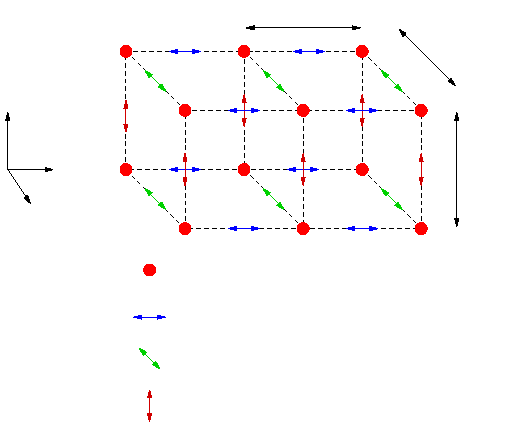
\includegraphics{fdtd_grid.pdf}%
\end{picture}%
\setlength{\unitlength}{4144sp}%
%
\begingroup\makeatletter\ifx\SetFigFont\undefined%
\gdef\SetFigFont#1#2#3#4#5{%
  \reset@font\fontsize{#1}{#2pt}%
  \fontfamily{#3}\fontseries{#4}\fontshape{#5}%
  \selectfont}%
\fi\endgroup%
\begin{picture}(3869,3327)(3541,-1288)
\put(6841,1649){$\delta y$}%
\put(3556,1244){z}%
\put(4006,704){x}%
\put(3826,344){y}%
\put(5806,1874){$\delta x$}%
\put(4996,-61){Pressure point}%
\put(4996,-421){Particle velocity x-direction}%
\put(4996,-781){Particle velocity y-direction}%
\put(4996,-1096){Particle velocity z-direction}%
\put(7066,704){$\delta z$}%
\end{picture}%
	\caption{The model of a continues line source where y axis is pointing towords the reader. (ref the book)}
		\label{fig:fdtd_cartesian_grid}
\end{figure}


The grid points is build up on positions there is descried as $(i\,\delta x,j\,\delta y,k\,\delta z)$ at time $t=l$, where $\delta x,\delta y,\delta z$ is the spatial discretization step \autoref{fig:fdtd_cartesian_grid} and $\delta t$ is the time spatial discretization step. $i,j,k$ is the discrete indices for the point in grid and $l\delta t$ is the discrete time index. For every axis, the component of the particle velocity have to be determined at position in \autoref{fdtd_component} at time $t=(l+\frac{1}{2})\delta t$.

\begin{equation}\label{fdtd_component}
\vec{v}= \begin{bmatrix}
v_x[(i\pm \frac{1}{2})\,\delta x,j\,\delta y,k\,\delta z]\\
v_y[i\,\delta x,(j\pm \frac{1}{2})\,\delta y,k\,\delta z]\\
v_z[i\,\delta x,j\,\delta y,(k\pm \frac{1}{2})\,\delta z]
\end{bmatrix}
\end{equation}

The following step is done to get the linearized equation for pressure and particle velocity in Cartesian grid and with air as medium. First \autoref{fdtd_euler} has to be rewritten to \autoref{fdtd_euler_rewrite_2}


\begin{subequations}\label{fdtd_euler_rewrite}
\begin{alignat}{2}
-\rho_0 \frac{\partial \vec{v}}{\partial t} &=\vec{\triangledown }p \label{fdtd_euler_rewrite_1}\\
-\rho_0 \frac{\partial \vec{v}}{\partial t} &=\frac{\partial p}{\partial x}\vec{x}+\frac{\partial p}{\partial y}\vec{y}+\frac{\partial p}{\partial z}\vec{z} \label{fdtd_euler_rewrite_2}
\end{alignat}
\end{subequations}


Second \autoref{fdtd_linear} has to be rewritten to \autoref{fdtd_linear_rewrite_2}

\begin{subequations}\label{fdtd_linear_rewrite}
\begin{alignat}{2}
- \frac{1}{\rho_0c^2} \frac{\partial p}{\partial t} &=\vec{\triangledown }v \label{fdtd_linear_rewrite_1}\\
- \frac{1}{\rho_0c^2} \frac{\partial p}{\partial t} &=\frac{\partial v_x}{\partial x}\vec{x}+\frac{\partial v_y}{\partial y}\vec{y}+\frac{\partial v_z}{\partial z}\vec{z}\label{fdtd_linear_rewrite_2}
\end{alignat}
\end{subequations}

The linearizing of \autoref{fdtd_euler_rewrite_2} is done with combining  




\autoref{fdtd_linear_rewrite_2} 



